\begingroup
	\pgfdeclarelayer{background layer}
	\pgfsetlayers{background layer,main}
	\tikzstyle{zero}=[circle,draw=black,fill=gray,inner sep=0pt,minimum size=2.5mm]
	\tikzstyle{one}=[circle,draw=black,fill=black,inner sep=0pt,minimum size=2.5mm]
	\tikzstyle{two}=[circle,draw=black,fill=white,inner sep=0pt,minimum size=2.5mm]
	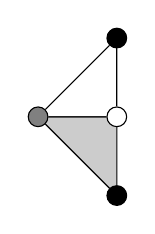
\begin{tikzpicture}
		\node (1) at (2,3) [two] {};
		\node (4) at (2,4) [one] {};
		\node (a) at (1,3) [zero] {};
		\node (d) at (2,2) [one] {};
		
		\begin{pgfonlayer}{background layer}
			\fill [black,opacity=0.2] (1,3)--(2,2)--(2,3)--(1,3);
		\end{pgfonlayer}
		
		\draw (1)-- (4);
		\draw (a)-- (d)-- (1)-- (a);
		\draw (a)-- (4)-- (1)-- (a);
	\end{tikzpicture}
	%\label{fig:eg_non_pure}
\endgroup